\section{Introduction}
\label{sec:introduction}

\begin{figure}[htb] \centering
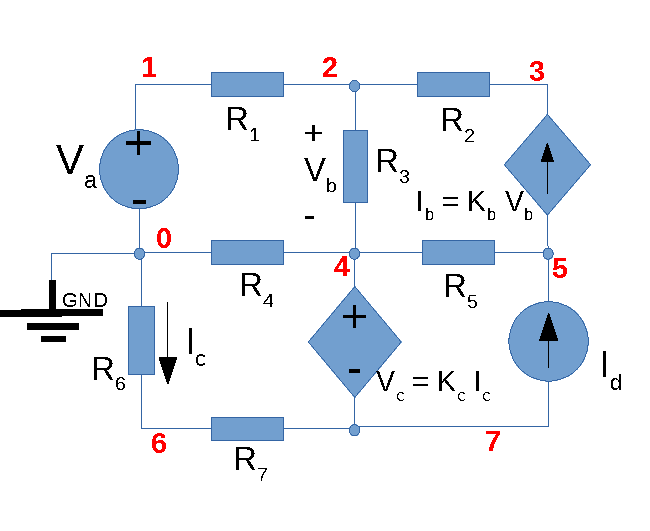
\includegraphics[width=0.4\linewidth]{rcm.pdf}
\caption{Nodal representation of the circuit.}
\label{fig:rc}
\end{figure}

\begin{table}[H]
  \centering
  \begin{tabular}{|l|r|}
    \hline    
    {\bf Name} & {\bf Value} \\ \hline
    R(1) & 1.015259 \\  \hline 
R(2) & 2.090689 \\  \hline 
R(3) & 3.108356 \\  \hline 
R(4) & 4.101243 \\  \hline 
R(5) & 3.033480 \\  \hline 
R(6) & 2.009605 \\  \hline 
R(7) & 1.005573 \\  \hline 
C & 1.015319 \\  \hlineVs & 5.026261 \\  \hlineKb & 7.161103 \\  \hlineKd & 8.185741 \\  \hline
  \end{tabular}
  \caption{Constants provided by Python. A variable  preceded by !! is of type {\it capacitance}
    and expressed in Farad ;a variable preceded by § is of type {\it resistence} and expressed in
    Ohm;a variable preceded by £ is of type {\it conductance} and expressed in
    Siemens; other variables are of type {\it voltage} and expressed in
    Volt.}
  \label{tab:op}
\end{table}

% state the learning objective 
The objective of this laboratory assignment is to find the natural, forced and total solution, with the use of a nodal analysis an the equivalent resistance, which will be used to plot the frequency response of the functions $v_c(f)$ and $v_6(f)$. The circuit can be seen in Figure ~\ref{fig:rc}. 



In section 2, a theoretical analysis of the circuit is presented. In section 5, the circuit is analyzed by simulation, and the results are compared to the theoretical results obtained in section 2. Finally, in section 6, we conclude our study.


